\chapter{Introduction to Egress and Ingress Scenarios in Selected CNI Plugins}
\label{cha:introScenarios}
In modern Kubernetes networking, managing traffic flow into and out of a cluster is crucial for performance and security. Different CNI plugins provide distinct mechanisms for controlling network traffic, each offering a unique approach to networking implementation. Understanding how traffic is managed in both ingress and egress scenarios is essential for improving security, optimizing performance, and enhancing overall network efficiency.

\section{Egress scenario: routing outgoing traffic via Egress Gateway}
\label{sec:egress}

The egress gateway can play a key role in a cluster's security. It can enforce routing all outgoing connections initiated within labeled pods through the gateway node. The node can route all outgoing traffic through a security system to scan each packet for potential threats, ensuring that outgoing traffic only accesses secure services outside the cluster.

The IT department of a financial company manages Kubernetes clusters in their local laboratory. The infrastructure is used to create a production-ready, efficient, and secure environment for financial services, where handling sensitive data and adhering to strict regulatory standards is critical. Leaving unmonitored critical traffic leaving the cluster can create vulnerabilities, potentially exposing the system to data exfiltration from financial applications. They decided to analyze all outgoing traffic from financial services pods using intrusion detection system (IDS) software. However, they also provide services that do not require such robust security. Redirecting every request to the traffic analyzer would add unnecessary overhead to exposed applications and cause higher latency. Cluster operators decided to leverage an egress gateway to route all outgoing traffic from financial services into a security tool to monitor and analyze packets. However, end users started complaining that their applications were showing errors like "503 Service Unavailable." The IT administrators began troubleshooting and concluded that the egress gateway was acting as a bottleneck in the cluster. They started searching online for solutions and decided to create separate gateways for each deployment of their services \cite{CalicoEgressDeploy}. End users stopped complaining about poor service availability.

\subsection{Egress gateway in selected CNI plugins}
\label{subsection:egressGateway}

Container Network Interface (CNI) plugins implement their own egress gateways, offering unique features. This section explores the capabilities of the Antrea and Cilium CNI plugins, focusing on how they handle outbound traffic and integrate with other networking components. Understanding these implementations is essential for Kubernetes operators to select the right CNI plugin for their specific requirements.


\subsubsection{Antrea}
\label{subsection:antreaEgress}

The Antrea Egress CRD (Custom Resource Definition) API is a resource that controls how pods in a cluster access external services. This resource specifies which egress IP should be used by selected pods. When a pod communicates with an external network, the traffic is routed through the node that has the specified egress IP (egress gateway). The source IP address of the traffic is then translated to the configured IP address \cite{AntreaEgressArch}.

\begin{figure}[tbh]
    \centering
    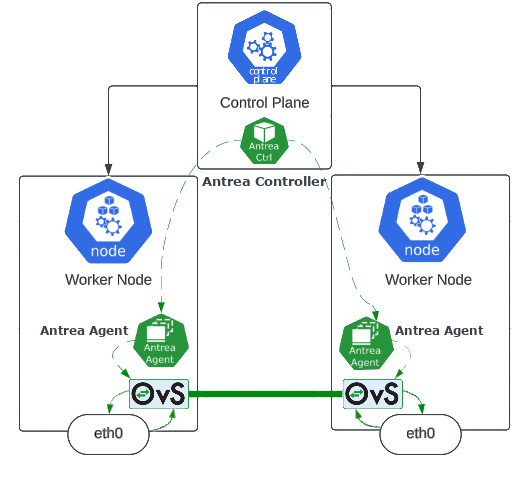
\includegraphics[width=0.6\columnwidth]{images/antrea_overview.png}
    \caption{Antrea Egress Architecture \cite{LucidApp}\cite{AntreaEgressArch}.}
    \label{fig:antreaEgressArch}
\end{figure}


Figure~\ref{fig:antreaEgressArch} shows the architecture of the communication flow when an egress gateway is configured in the Antrea CNI. When a pod running on a Kubernetes node tries to access an external service (assuming it is labeled to route its outbound traffic through the egress node), the traffic is tunneled (through OvS) to the gateway node, and the Antrea Agent performs SNAT. After translation, the next network peer that communicates with the egress gateway will see its IP as the source IP, instead of the IP address of the pod \cite{AntreaEgressArch} \cite{AntreaSNAT} \cite{AntreaArch}.

Let's explain the egress configuration YAML from Listing~\ref{lst:yamlAntreaEgress} \cite{AntreaEgressArch}:
\begin{itemize}
    \item Antrea allows matching the pods that route through the egress gateway based on two criteria:

    \begin{enumerate}
        \item namespaceSelector -- specifies which pods within the specified namespace should redirect outbound traffic.
        \item podSelector -- selects pods with the specified labels. For example, it can match pods labeled with role=web to redirect traffic.
    \end{enumerate}

    \item egressIP -- specifies SNAT IP address of an egress gateway, to which traffic is tunneled
    \item externalIPPool -- name of externalIPPool resource which contains pool of IP addresses to allocate if egressIP is not set
\end{itemize}

It is possible to configure a failover egress gateway node using Antrea. To do this, egressIP and externalIPPool must be set (with egressIP being part of externalIPPool). When the current egress gateway stops working, another node within the externalIPPool will be selected. This infrastructure, with a failover service, is part of a high-availability setup for production environments (useful for the previously mentioned IT department) \cite{AntreaEgressArch}.


\begin{listing}[htb]
    \centering
    \caption{Egress resource example \cite{AntreaEgressArch}.}
    \begin{minted}[gobble=4, frame=single, linenos, fontsize=\scriptsize]{yaml}
    apiVersion: crd.antrea.io/v1alpha2
    kind: Egress
    metadata:
        name: egress-prod-web
    spec:
        appliedTo:
        namespaceSelector:
            matchLabels:
            env: prod
        podSelector:
            matchLabels:
            role: web
        egressIP: 10.10.0.8
        externalIPPool: prod-external-ip-pool
    status:
        egressNode: node01
    \end{minted}
    \label{lst:yamlAntreaEgress}
\end{listing}

The ExternalIPPool resource from Listing~\ref{lst:yamlAntreaExternalIPPool} can be configured with the following fields \cite{AntreaEgressArch}:

\begin{itemize}
    \item ipRanges -- IP pools range can be configured using a pair of IP (start and end), or by setting CIDR (Classless Inter-Domain Routing) range
    \item nodeSelector -- will apply only on nodes specified by this field, e.g., nodes labeled with network-role: egress-gateway
\end{itemize}

\begin{listing}[htb]
    \centering
    \caption{ExternalIPPool resource example \cite{AntreaEgressArch}.}
    \begin{minted}[gobble=4, frame=single, linenos, fontsize=\scriptsize]{yaml}
    apiVersion: crd.antrea.io/v1alpha2
    kind: ExternalIPPool
    metadata:
        name: prod-external-ip-pool
    spec:
        ipRanges:
            - start: 10.10.0.2
              end: 10.10.0.10
            - cidr: 10.10.1.0/28
        nodeSelector:
        matchLabels:
            network-role: egress-gateway
    \end{minted}
    \label{lst:yamlAntreaExternalIPPool}
\end{listing}
  


\subsubsection{Cilium}
\label{subsection:ciliumEgress}

To take advantage of Cilium's egress gateway features, eBPF masquerading must be enabled, and the node's kube-proxy component must be replaced with Cilium's implementation \cite{CiliumEgressGateway}. As shown in Figure~\ref{fig:ciliumEgressArch}, the Cilium agent injects routing information into eBPF maps within the kernel (relying on kernel support for eBPF features). Traffic from worker nodes is redirected to the egress gateway node, where it is SNATed and leaves the cluster. These routes, defined by Cilium policies configured in the control plane, ensure that every node is aware of which pods should redirect traffic to the designated egress node \cite{CiliumEgressGateway}. For node-to-node communication, Cilium encapsulates all traffic using UDP-based VXLAN or Geneve protocols \cite{CiliumRouting}.

\begin{figure}[tbh]
    \centering
    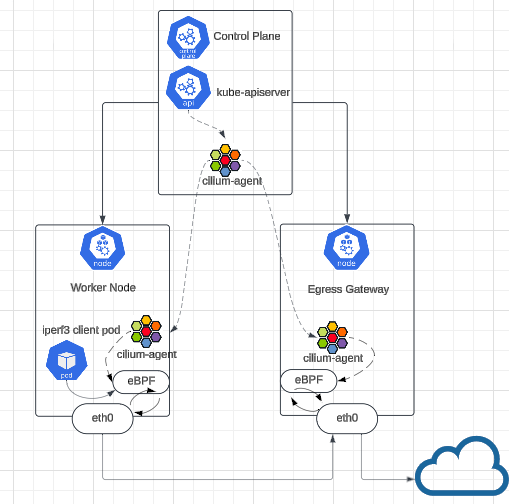
\includegraphics[width=0.9\columnwidth]{images/cilium_egress.png}
    \caption{Cilium Egress Architecture \cite{K8sIcons}\cite{LucidApp}\cite{CloudIcon2}\cite{CiliumEgressGatewayBlog}.}
    \label{fig:ciliumEgressArch}
\end{figure}

Similar to Antrea egress resources, Cilium has its own CiliumEgressGatewayPolicy present on Listing~\ref{lst:yamlCiliumEgressGatewayPolicy} \cite{CiliumEgressGateway}:

Cilium allows matching the traffic that route through the egress gateway by \cite{CiliumEgressGateway}:
\begin{itemize}
    \item podSelector -- matching pods based of used selector, like previous matching labels in Antrea, or by matching expressions (key operator, values). More than one podSelector can be used
    \item destinationCIDRs -- an app in pod is requesting some external service, if this resource is match by defined CIDR, the request is routed to egress gateway. For 0.0.0.0/0 all traffic is outgoing by egress gateway. Setting excludedCIDRs is possible to exclude some IPs.
\end{itemize}

Selecting an egress gateway can be done in three ways: by matching node labels, using IP address in egressIP field (as in Antrea) or by interface name \cite{CiliumEgressGateway}. 

\begin{listing}[htb]
    \centering
    \caption{Egress resource example \cite{AntreaEgressArch}.}
    \begin{minted}[gobble=4, frame=single, linenos, fontsize=\scriptsize]{yaml}
    apiVersion: cilium.io/v2
    kind: CiliumEgressGatewayPolicy
    metadata:
    name: egress-sample
    spec:
    selectors:
    - podSelector:
        matchLabels:
            org: empire
            class: mediabot
            io.kubernetes.pod.namespace: default
        matchExpressions:
            - {key: testKey, operator: In, values: [testVal]}
            - {key: testKey2, operator: NotIn, values: [testVal2]}
    destinationCIDRs:
    - "0.0.0.0/0"
    excludedCIDRs:
    - "192.168.1.0/24"
    egressGateway:
        nodeSelector:
        matchLabels:
            node.kubernetes.io/name: a-specific-node
        egressIP: 10.168.60.100
    \end{minted}
    \label{lst:yamlCiliumEgressGatewayPolicy}
\end{listing}


Both Antrea and Cilium allow us to configure an egress gateway in multiple ways. Cilium offers more flexibility in defining which traffic should be routed through the egress gateway. Unlike Antrea, Cilium can specify traffic by destination CIDR. While Cilium provides more capabilities for matching egress traffic, Antrea's implementation allows for the creation of a failover node, which will route traffic if the primary one fails. Creating a high-availability egress gateway in Cilium is possible only with the enterprise, paid version of the plugin. Additionally, Cilium leverages eBPF, which is designed for large-scale clusters \cite{CiliumOverview}. It is not clear which egress gateway CNI implementation is the best to use, as each has its advantages and drawbacks. In the next section, both gateways will be evaluated using networking tools in a local environment.




\section{Ingress scenario: splitting incoming traffic via Gateway API}
\label{sec:ingress}

The Gateway API, as a successor to the Ingress object, provides enhanced features for traffic management and introduces a role-oriented approach to separate Kubernetes user and operator concerns. It supports traffic splitting, header modification, and URL rewriting. Additionally, the Gateway API supports key protocols such as HTTP, HTTPS, TCP, UDP, and gRPC. With its wide range of features, it can be used in various ways \cite{CiliumGatewayAPIBlog}.

%---------------------------------------------------------------------------
\subsubsection{Canary Deployment}
\label{subsubsection:canary}

Canary Deployment is one of the most common methods used to roll out a new application version to end users, ensuring that everything is working as expected before the full release. The core idea is to release new versions of software only to a small group of users, leaving most users unaware of the new release \cite{Canary}.

This is where the traffic splitting feature of the Gateway API can be used \cite{CiliumTrafficSplitting}. There are typically five stages in the deployment process \cite{Canary}:

\begin{itemize}
    \item Initial state -- The stable version of the application is served.
    \item Canary stage -- The updated version of the application is visible only to 5\% of users. As some users interact with the newly provisioned software, the most common errors should be visible (if any).
    \item Early stage -- The second stage of canary deployment, where the new app is available to 25\% of total connections. At this point, less frequent bugs may be observed.
    \item Mid stage -- The app is available to 50\% of end users. Half of the traffic is routed to the latest version of the app. At this point, the performance of the rolled-out software is monitored.
    \item Late stage -- Most of the traffic (75\%) is handled by the recent version of the application. This stage precedes the full release of the new software.
    \item Full stage -- 100\% of users are served the new application version.
\end{itemize}

If any anomalies are detected during any stage of the canary deployment, the new application version should be immediately rolled back.

The Gateway API is not designed for software deployment and does not have capabilities for rolling back applications automatically. In this usage, the gateway is used only for weighted traffic splitting.

%---------------------------------------------------------------------------

\subsubsection{Traffic Mirroring with Gateway API}
\label{subsubsection:mirroring}

A company is offering a weather API, but not all endpoints are publicly available. Some features are secured and paid. Securing these paid interfaces is not as critical as securing more sensitive and confidential data. Recently, the company decided to start analyzing incoming traffic on these secured endpoints to ensure that only authorized requests are being handled. However, the company does not have the infrastructure capabilities to analyze all incoming traffic for these endpoints. As their services are HTTP-based inside a Kubernetes cluster, they can take advantage of the Gateway API’s traffic splitting feature. The security team decided to route 40\% of the incoming traffic to a traffic analyzer to evaluate whether and how requests might bypass the paywall. The cluster management team (acting as both infrastructure providers and cluster operators, according to the roles in the Gateway API model) decided to split the traffic using the Gateway API, as they need general usage of the API Gateway (since the company offers RESTful APIs). Pure traffic splitting is not sufficient in this case because all incoming traffic must be handled in response. The solution is to split 40\% of the traffic to a different Kubernetes service, mirror the traffic to the analyzer, and then route it back to the pod containing the application. While the cluster managers implement the second deployment to mirror requests to the traffic analyzer, the app developers created an HTTPRoute object with appropriate weights for each of the services. Figure~\ref{fig:mirroringImg} shows how the cluster infrastructure might look in this case.


\begin{figure}[H]
    \centering
    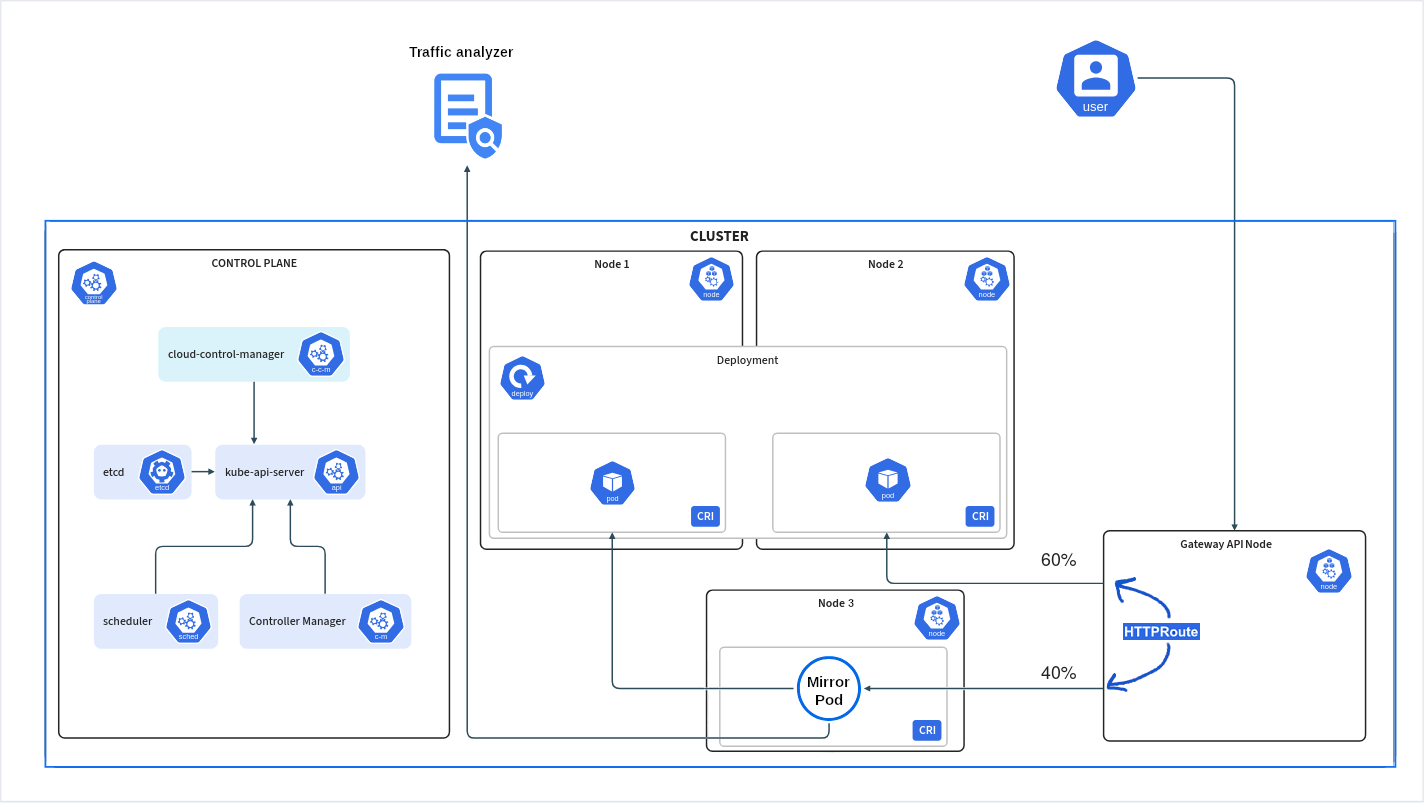
\includegraphics[width=1\columnwidth]{images/ingress.png}
    \caption{Example Kubernetes cluster with traffic mirroring \cite{KubernetesArch}\cite{K8sIcons}\cite{LucidApp}.}
    \label{fig:mirroringImg}
\end{figure}

%---------------------------------------------------------------------------

\subsection{Traffic splitting in selected CNI plugins}
\label{subsection:trafficSplitting}

Unfortunately, the Antrea plugin does not provide an implementation of the Gateway API. In fact, Cilium is the only CNI plugin that offers this functionality. To evaluate the cluster networking implementation with Antrea CNI, the NGINX Gateway Fabric can be used instead.



%---------------------------------------------------------------------------
\subsubsection{Antrea + NGINX}
\label{subsection:antreaIngress}

Figure~\ref{fig:canaryAntreaImg} shows an example cluster where the Gateway API is configured to work in the canary stage. Antrea CNI is installed, and the antrea-ctrl and antrea-agent pods are deployed on the nodes. OvS tunneling among nodes is set up \cite{Antrea}. On the control plane node, the NGINX Gateway API is deployed as a pod \cite{NGINX}. This differs from Cilium, where the Gateway API is not run as a single pod \cite{CiliumGatewayAPI}. In this setup, traffic is processed by the NGINX Gateway API pod, while Antrea handles the networking stack, integrating with NGINX to manage traffic routing.

\begin{figure}[H]
    \centering
    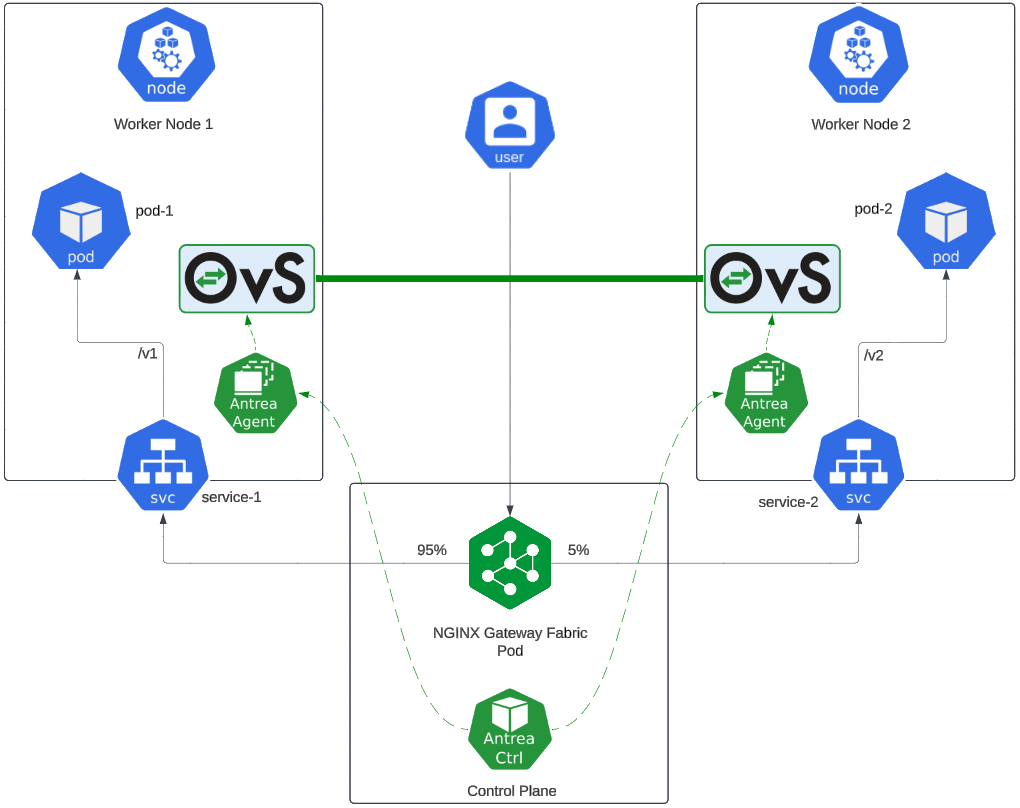
\includegraphics[width=1\columnwidth]{images/antrea-nginx.png}
    \caption{Example Kubernetes cluster with Antrea CNI and NGINX Gateway Fabric in canary stage of canary deployment \cite{KubernetesArch}\cite{K8sIcons}\cite{LucidApp}\cite{AntreaEgressArch}.}
    \label{fig:canaryAntreaImg}
\end{figure}

\begin{listing}[htb]
    \centering
    \caption{Egress resource example \cite{AntreaEgressArch}.}
    \begin{minted}[gobble=4, frame=single, linenos, fontsize=\scriptsize]{yaml}
    apiVersion: gateway.networking.k8s.io/v1
    kind: HTTPRoute
    metadata:
        name: current-weather-route
    spec:
        parentRefs:
        - name: nginx-gw
        rules:
        - matches:
            - path:
                type: PathPrefix
                value: /getCurrentWeather
            backendRefs:
            - kind: Service
                name: current-weather-pod-1
                port: 8080
                weight: 95
            - kind: Service
                name: current-weather-pod-2
                port: 8090
                weight: 5
    \end{minted}
    \label{lst:yamlAntreaIngressCanaryHTTPRoute}
\end{listing}
%---------------------------------------------------------------------------

\subsubsection{Cilium}
\label{subsection:ciliumIngress}

In Figure~\ref{fig:ciliumDataflow}, an example canary cluster stack using the Cilium plugin is presented. The arrows represent the real data traffic flow, while the dashed arrows indicate the configuration flow. The HTTPRoute resources are pulled by the cilium-agent, which prepares the configuration and injects it into the Envoy proxy and eBPF. When Envoy receives an incoming request, it understands the traffic-splitting ratio and decides whether to route the traffic to a local pod or to a different pod, as specified in the HTTPRoute configuration \cite{CiliumComponents}. The HTTPRoute resource for the Cilium Gateway API will look almost exactly the same as in Listing~\ref{lst:yamlAntreaIngressCanaryHTTPRoute}, with the only difference being the parentRefs name, which defines which Gateway is being used.

\begin{figure}[H]
    \centering
    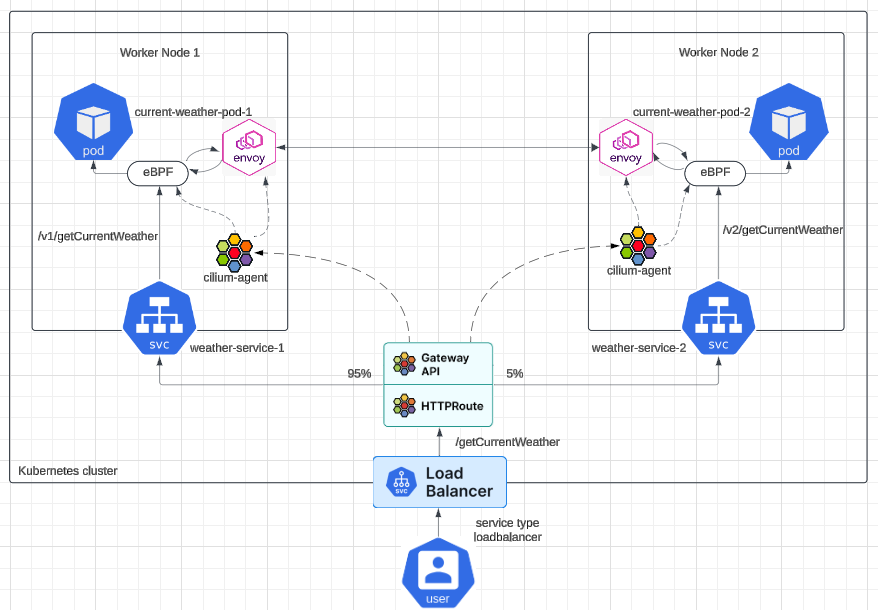
\includegraphics[width=1\columnwidth]{images/cilium_dataflow.png}
    \caption{Example Kubernetes cluster with Cilium CNI in canary stage of canary deployment \cite{K8sIcons}\cite{LucidApp}\cite{CiliumEgressGatewayBlog}.}
    \label{fig:ciliumDataflow}
\end{figure}

%---------------------------------------------------------------------------